%
\documentclass[10pt,a4paper]{article}


\usepackage{array}
\usepackage{subfigure}
\usepackage{graphicx}
\usepackage{amssymb}
\usepackage{amsmath}
\usepackage{cite}
\usepackage{color}
\usepackage{url}
\usepackage[lined,linesnumbered,ruled,norelsize]{algorithm2e}
\usepackage{listings}
\lstset{
  language=Octave, 
  basicstyle=\footnotesize, 
  frame=single, 
  showspaces=false, 
  showstringspaces=false}
\date{}




\begin{document}

\title{Technical Report 8: K-means}

\maketitle

We illustrate the image with the number of its colors reduced by K-means algorithms in Fig. \ref{fig:rel}
%
%
    \begin{figure}[htb!]
       \begin{center}
       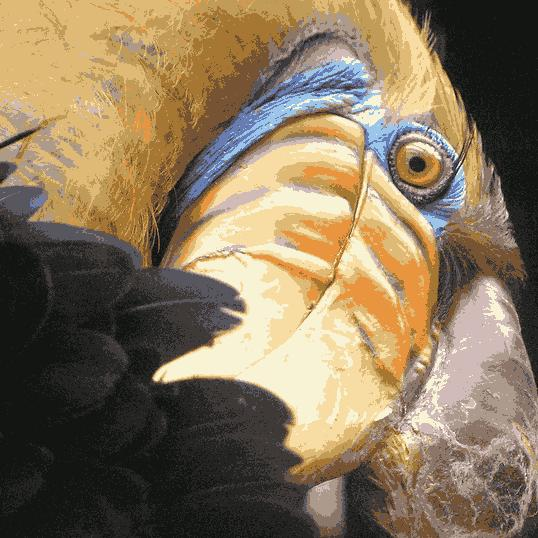
\includegraphics[width=.9\columnwidth]{bird_kmeans}
       \end{center}
       \caption{The results of applying K-means algorithm to the image.}
       \label{fig:rel}
    \end{figure}
%
The color spectrum is given in Fig. \ref{fig:spc}.
%
\begin{figure}[htb!]
       \begin{center}
       
\includegraphics[width=.9\columnwidth]{colors}
       \end{center}
       \caption{Color spectrum.}
              \label{fig:spc}
    \end{figure}
%



\end{document}








  \end{lstlisting}
  %


